\documentclass[twoside,11pt]{article}
\usepackage{jmlr2e}
\usepackage{graphicx}
\graphicspath{ {./images/} }
\usepackage{enumitem}
\newlist{mylistenv}{enumerate}{3}
\newenvironment{mylist}[1]{%
	\setlist[mylistenv]{label=#1\arabic{mylistenvi}.,ref=#1\arabic{mylistenvi}}%
	\setlist[mylistenv,2]{label=#1\arabic{mylistenvi}.\arabic{mylistenvii}.,ref=#1\arabic{mylistenvi}.\arabic{mylistenvii}}%
	\setlist[mylistenv,3]{label=#1\arabic{mylistenvi}.\arabic{mylistenvii}.\arabic{mylistenviii}.,ref=#1\arabic{mylistenvi}.\arabic{mylistenvii}.\arabic{mylistenviii}}%
	\renewenvironment{mylist}{\begin{mylistenv}}{\end{mylistenv}}
	\begin{mylistenv}%
	}{%
	\end{mylistenv}%
}
\newcommand\tab[1][1cm]{\hspace*{#1}}

% Definitions of handy macros can go here

\newcommand{\dataset}{{\cal D}}
\newcommand{\fracpartial}[2]{\frac{\partial #1}{\partial  #2}}


\firstpageno{1}

\begin{document}

\title{Project 4: Networks for Classification and Regression}

\author{\name Sarah Wilson 
	   \email swi1s117@jhu.edu \\
	   \phone 303-921-7225 \\
       \addr Engineering Professionals Computer Science\\
       Johns Hopkins University\\
       Baltimore, MD 21218, USA} 

\maketitle


\section{Introduction}
\hspace*{10mm} Neural Networks are collection of algorithms that are taught the underlying patterns in a data set through a process of supervised learning. Neural Networks operate using a process that is similar to the human brain, they contain simple processing nodes, called neurons that are connected in layers. These layers contain weights that determine an output based on a given input. The basis of an understanding of Neural Networks actually starts with Linear Regression.\\ 
\hspace*{10mm} Linear Regression is a supervised Machine Learning algorithm that can be applied to Regression problems. Linear Regression assumes there is some sort of linear relationship between the input data and the output value that can be represented by a line or plane of best fit between the inputs and the output. Linear Regression is meant for continuous outputs, when Classification tasks are required (tasks that have outputs with class labels), then the concepts of linear regression can be applied, but instead the Sigmoid function is used, hence the name Logistic Regression. The sigmoid function is able to take classifiers that are not numeric and map them to values between 0 and 1. Linear and Logistic regression are the basic concepts that build the foundation for Neural Networks. Neural Networks can be thought of as a series of Logisitc regression tasks that happen across many layers and nodes. Neural Networks can also be augmented through the use of developing an Auto Encoder. The Auto Encoders are trained such that an output pattern to a network always matches the input pattern. The Auto Encoder process can be thought of a method to fine tune the weights feeding the prediction output from a Neural Network.\\
\hspace*{5mm} The problem statement presented in this paper is to understand an implement three major categories of networks; Linear, Feed-Forward Back Propagation and  Feed-Forward Back Propagation with an Auto Encoder. For the Linear Network: a Linear Regression will be applied to Regression problems while a Logistic Regression will be applied to the Classification Problems.\\
\hspace*{5mm} The hypothesis of this report is that the  Feed-Forward Network with an Auto Encoder will perform better than the Feed-Forward Back Propagation and Linear regression approaches on both the Classification and Regression problems. The reason for this hypothesis is that the Auto Encoder builds upon the Linear Regression and basic Neural Regression. Both Linear Regression and Neural Networks rely on updating weight based on the error between the predicted output and the actual output of a training set. The Auto Encoder improves upon this process by trying to learn and mimic the input pattern of the data and apply that to the output or predicted value. This extra encoding and decoding steps, serve to fine tune the weights feeding the neural network. The hypothesis is based around the concept that fine tuned weights should out preform coarsely tuned weights in making predictions based on new input data to the network. The results from experiments ran on the provided data sets will be discussed and presented against the outlined hypothesis.\\
\hspace*{5mm} Section 1 has provided the introduction, problem statement and hypothesis in regards to three major learning algorithms that will be explored. Section 2 will provide an in-depth explanation of the algorithms. Section 3 will present the results obtained by the different algorithms. Section 4 will discuss the results that were obtained and compare them to the hypothesis that was outlined in the introduction. This report will conclude in Section 5 with a discussion of lessons learned and areas of possible future work.\\


\section{Algorithms and Experimental Methods}
\hspace*{10mm} Regression is an a problem solving approach in Machine Learning that models a target predictor based on independent variables or values.  Linear Regression and Logistic Regression both are discriminant-based approaches that do not care about estimating the densities inside a particular class region, instead the discriminant-based approach aims to estimate the boundaries between the class regression. Linear and Logistic Regression provide a simple model that is the form of a linear formula, in order to determine the class of a particular observation from the data. The output of the model is a weighted sum of the input attributes or features. The magnitude of the weight applied against each feature, shows the importance of that feature towards the overall prediction. The weights are learned by the model during training. Linear Regression is used on Regression problems because the data that is being predicted is continuous. This Linear model will not work for Classification problems, as the output of the linear model would be a real value, when in Classification a class label is desired. Logistic Regression is used for Classification problems, as it maps the output of the weight sum presented in Linear Regression and maps it to a non-linear function that ensures the outputs are between 0 and 1. The function used to achieve this is the Sigmoid or Logistic function.\newline
\hspace*{10mm} The objective of training in both Linear and Logistic Regression is to determine the weights that will be used in the final model. The weight coefficients can be determined using the process of Gradient Descent. The general procedure for applying Gradient Descent is to first calculate the prediction based on the current weight coefficients and then calculate new coefficients based off the error in the prediction. This process is repeated until the coefficients are deemed accurate enough, the process used in this paper to determine the prediction is accurate enough will be to determine that the error has dropped to a desirable enough level. At this point the model can be considered trained and will be evaluated for performance on the test data set.

The general algorithm steps for Linear and Logistic Regression are outlined below:\newline
For each Feature (\textit{j}) in the Domain(\textit{d}) of the Data Set\\
\tab Set $W_j$ to a random value between -0.01 and 0.01\\
Repeat the Following Steps Until the Error has Converged to a Value ()\\
\tab For each Feature (\textit{j}) in the Domain(\textit{d}) of the Data Set\\
\tab \tab $\delta W_j$ = 0\\
 \tab For each Feature (\textit{j}) in the Domain(\textit{d}) of the Data Set\\
 

\newpage
{\noindent}{\bf Data Sets}\newline
The following data sets were used during the classification and regression tasks for this project.\newline
{\bf Breast Cancer}\newline
Description: \newline
Task: Classification\newline
Predictor: Diagnosis (Malignant or Benign)\newline
Link:\newline \url{https://archive.ics.uci.edu/ml/datasets/Breast+Cancer+Wisconsin+%28Original%29}\newline
{\noindent}\textbf{Car Evaluation}\newline
Description:\newline
Task: Classification\newline
Predictor: Car Evaluation (Unacceptable, Acceptable, Good, Very Good)\newline
Link: \newline
\url{https://archive.ics.uci.edu/ml/datasets/Car+Evaluation}\\
{\noindent}\textbf{Congressional Vote}\newline
Description: 1984 United Stated Congressional Voting Records\newline
Task: Classification \newline
Predictor: Party (Republican / Democrat) \newline
Link: \newline
\url{https://archive.ics.uci.edu/ml/datasets/Congressional+Voting+Records}\newline
{\noindent}\textbf{Albalone}\newline
Description: Physical measurements of Albalone\newline
Task: Regression\newline
Predictor: Rings (int)\newline
Link: \newline
\url{https://archive.ics.uci.edu/ml/datasets/Abalone}\newline
{\noindent}\textbf{Computer Hardware}\newline
Description: Relative CPU performance data.\newline
Task: Regression\newline
Predictor: PRP\newline
Link: \newline
\url{https://archive.ics.uci.edu/ml/datasets/Computer+Hardware}\newline
{\noindent}\textbf{Forest Fires}\newline
Description: Forest Fire burn area data\newline
Task: Regression\newline
Predictor: Area (float)\newline
Link: \newline
\url{https://archive.ics.uci.edu/ml/datasets/Forest+Fires}\newline
	
\newpage

\section{Results}
Tables 1-3 display the results from Classification Tasks: the Breast Cancer, Car Evaluation and Congressional Vote data sets while running all three algorithms. Tables 4-6 display the results from the Regression Tasks: the Albalone, Computer Hardware and Forest Fire data sets while running all three algorithms. Each algorithm was tuned prior to being run on the full experiment set and optimal values were chosen out of that tuning process for the Learning Rate and the Convergence Factor. These tables show the results obtained during each fold of the \textit{k}-fold validation process. The results from each iteration of the tuning process was omitted from this report for brevity. The error used is Classification error and can be described as the Number of Times the Prediction was Wrong / Total Number of Comparisons. This error was averaged across the 5 folds to provide the Average Classification Error against each of the Classification data sets. The error used for Regression Tasks was the Mean Root Squared Error. This error was averaged across the 5 folds to provide the Average Mean Root Squared Error against each of the Regression data sets.\newline


\begin{table}[h]
		\centering
		\caption{Car Evaluation:Linear Networks - Experimental Results}
		\label{tab:table1}
		%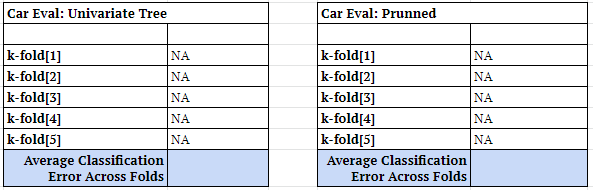
\includegraphics[scale=.7]{CarEval_Results}\newline
\end{table}

\begin{table}[h]
		\centering
		\caption{Breast Cancer: Linear Networks - Experimental Results}
		\label{tab:table2}
		%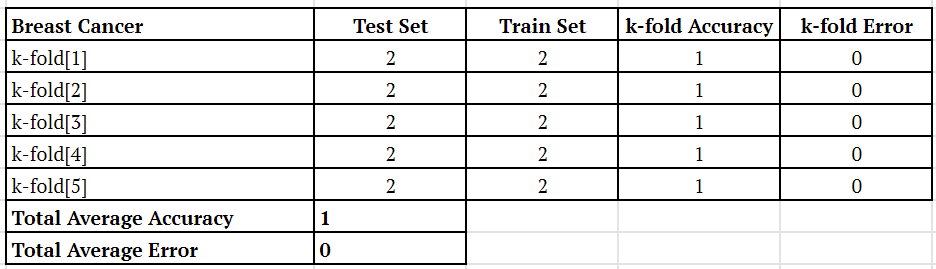
\includegraphics[scale=.7]{BC_Results}\newline
\end{table}
\newpage

\begin{table}[h]
		\centering
		\caption{Congressional Vote: Linear Networks - Experimental Results}
		\label{tab:table3}
		%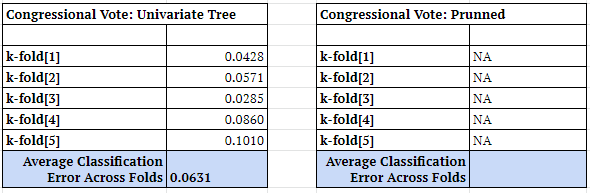
\includegraphics[scale=.7]{CongVote_Results}\newline
\end{table}

\begin{table}[h]
	\centering
	\caption{Albalone: Linear Networks - Experimental Results}
	\label{tab:table4}
	%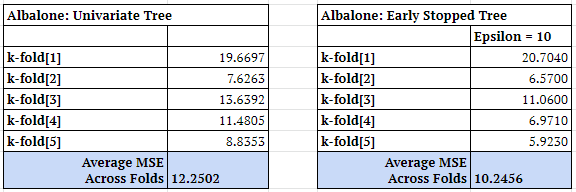
\includegraphics[scale=.7]{Albalone_Results}\newline
\end{table}

\begin{table}[h]
	\centering
	\caption{Computer Hardware: Linear Networks - Experimental Results}
	\label{tab:tale5}
	%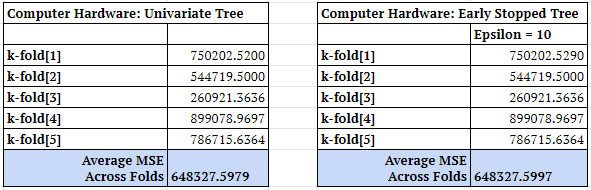
\includegraphics[scale=.7]{CompHardware_Results}\newline
\end{table}

\begin{table}[h]
	\centering
	\caption{Forest Fires: Linear Networks - Experimental Results}
	\label{tab:table6}
	%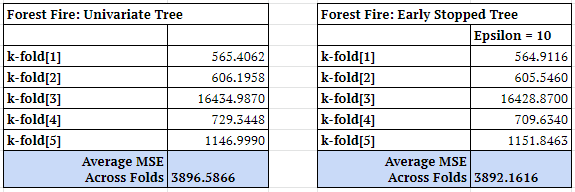
\includegraphics[scale=.7]{ForestFire_Results}\newline
\end{table}

\newpage
\newpage


\section{Discussion}
\hspace*{10mm} The hypothesis presented in this report was that the  Feed-Forward Network with an Auto Encoder will perform better than the Feed-Forward Back Propagation and Linear regression approaches on both the Classification and Regression problems.\\
\hspace*{10mm} Looking at the classification data sets,  \\

\hspace*{10mm} Looking at the Regression data sets,\\


\section{Conclusion}
\hspace*{10mm} Overall there seemed to be some trends that supported the general hypothesis. \newline

\hspace*{10mm} The .\newline

\hspace*{10mm} A suggested area of future work, after fixing basic implementation details, would be to explore as part of the tuning process the shape of the network. In the experiment the Neural Network that was built for the algorithm that included and input layer, 2 hidden layers and an output layer. This network could have been built with a different number of hidden layers and a variable number of nodes with in those hidden layers, that could have lead to different results. That structure of the network is an area that could be looked into for future work. \newline

\section{References}
1. Alpaydin, E. (2004). Introduction to machine learning (Oip). Mit Press. 

\newpage


\end{document}